\documentclass[a4paper,12pt]{article}

\usepackage[utf8]{inputenc} 
\usepackage{amsmath}
\usepackage[a4paper, margin=0.9in]{geometry} % Adjust the margin here
\usepackage{multirow}
\usepackage{graphicx}
\usepackage{tikz}
\usepackage{wrapfig}
    
\begin{document}

\section*{Question 1}
Consider a system of three point particles, each having an identical mass $m$, with their positions defined by time-dependent vectors,
\begin{equation*}
    \vec r_{1}~=~(at^2,~vt,~0),~\vec r_{2}~=~(vt,~at^2,~b),~\vec r_{3}~=~(0,~b,~at^2), 
\end{equation*}
where $a$, $b$, and $v$ are positive constants.
\begin{itemize}
    \item[\textbf{a.}] Find the total external force acting on this system. --- \textit{0.4 points}
    \item[\textbf{b.}] Find the total torque acting on this system concerning the origin of the coordinate system. --- \textit{0.4 points}
    \item[\textbf{c.}] Based on the results from parts (a) and (b), determine if total linear momentum and total angular momentum are conserved. --- \textit{0.2 points}
\end{itemize}

\section*{Question 2}
The equation of motion of a damped oscillator is given as $x(t)=e^{-\beta t}x_0\cos{\left(\omega_1 t\right)}$. How long does it take for the damped oscillator to halve the amplitude of the oscillation? 
(Givens: $\ln2\approx 0.7$, $m=~1\text{kg}$, $b=1.4~\text{kg/s}$) --- \textit{1 point}

\section*{Question 3}
For a given central force $f(r)$ the orbit of a particle of mass $\mu$ can be calculated by integrating the following differential equation,
\begin{equation*}
    \dfrac{d^2}{d\theta^2}\left(\frac{1}{r}\right)+\frac{1}{r}=-\frac{\mu}{l^2}r^2f(r)
\end{equation*}
where $l$ is the angular momentum of the particle. The particle follows an orbit given by $1+\epsilon\cos\theta=\alpha/r$, where $\alpha\equiv \frac{l^2}{\mu k}$ and $\epsilon \equiv \sqrt{1+\frac{2El^2}{\mu k^2}}$ are constants.

\begin{itemize}
    \item[\textbf{a.}] Find the force law $f(r)$ for the central force in terms of $k$ and $r$. --- \textit{0.8 points}
    \item[\textbf{b.}] Find the potential $U(r)$ associated with $f(r)$. --- \textit{0.2 points}
\end{itemize}

\section*{Question 4}
\begin{wrapfigure}{r}{0.35\textwidth}
    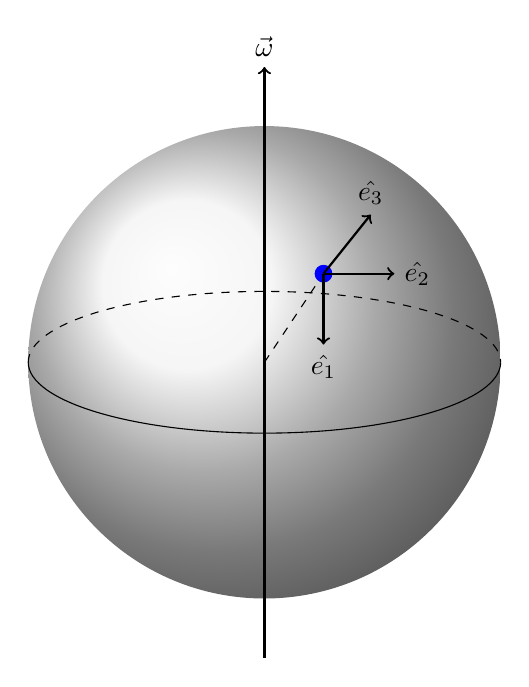
\begin{tikzpicture}[scale=1.5]
        % Draw the sphere
        \shade[ball color=gray!10] (0,0) circle (2cm);
        % Draw the axis of rotation
        \draw[thick,->] (0,-2.5) -- (0,2.5) node[above] {$\vec{\omega}$};
        % Draw the equator
        \draw (-2,0) arc (180:360:2 and 0.6);
        \draw[dashed] (-2,0) arc (180:0:2 and 0.6);
        \draw[dashed] (0,0) -- (0.5,0.75);
        % Draw the point particle
        \filldraw[blue] (0.5,0.75) circle (2pt);
        \draw[thick,->] (0.5,0.75) -- (0.9,1.25) node[above] {$\hat{e_3}$};
        \draw[thick,->] (0.5,0.75) -- (1.1,0.75) node[right] {$\hat{e_2}$};
        \draw[thick,->] (0.5,0.75) -- (0.5,0.15) node[below] {$\hat{e_1}$};
    \end{tikzpicture}
\end{wrapfigure}
In the figure, the earth's rotation about its axis with angular velocity $\vec{\omega}$ is shown. The unit vectors $\hat{e}_1$, $\hat{e}_2$, and $\hat{e}_3$ are local unit vectors on the Earth's surface, where $\hat{e}_3$ is perpendicular to the surface, while $\hat{e}_1$ and $\hat{e}_2$ lie on the surface. The component of $\vec{\omega}$ along the $\hat{e}_3$ direction is $\omega_z$. A particle of mass $m$ is projected horizontally with an initial velocity $\vec{v}=v_0\hat{e}_2$ from the point indicated in the figure. Assume the Earth is a perfect sphere with radius $R$ and neglect air resistance.

\textbf{a.} Determine the direction and magnitude of the Coriolis force. --- \textit{0.6 points}

\textbf{b.} Determine the equations of motion in $\hat{e}_1$ and $\hat{e}_2$ directions by considering only the Coriolis force and velocity $\vec{v}$, neglecting free-fall which is in $-\hat{e}_3$ direction. --- \textit{0.4 points}

(Given: Coriolis force $\vec{F}_c = -2m \vec{\Omega} \times \vec{v}$)

\end{document}
